DPC++ provides a rich set of SYCL built-in functions with respect to various data types. These built-in functions are available in the sycl namespace on host and device with low-, medium-, and high-precision support for the target devices based on compiler options, for example, the -mfma, -ffast-math, and -ffp-contract=fast provided by the DPC++ compiler. These built-in functions on host and device can be classified as in the following:\par

\begin{itemize}
	\item Floating-point math functions: asin, acos, log, sqrt, floor, etc. listed in Figure 18-2.
	\item Integer functions: abs, max, min, etc. listed in Figure 18-3.
	\item Common functions: clamp, smoothstep, etc. listed in Figure 18-4.
	\item Geometric functions: cross, dot, distance, etc. listed in Figure 18-5.
	\item Relational functions: isequal, isless, isfinite, etc. listed in Figure 18-6.
\end{itemize}

If a function is provided by the C++ std library, as listed in Figure 18-8, as well as a SYCL built-in function, then DPC++ programmers are allowed to use either. Figure 18-1 demonstrates the C++ std::log function and SYCL built-in sycl::log function for host and device, and both functions produce the same numeric results. In the example, the built-in relational function sycl::isequal is used to compare the results of std:log and sycl:log.\par

\hspace*{\fill} \par %插入空行
Figure 18-1. Using std::log and sycl::log
\begin{lstlisting}[caption={}]
constexpr int size = 9;
std::array<double, size> A;
std::array<double, size> B;

bool pass = true;

for (int i = 0; i < size; ++i) { A[i] = i; B[i] = i; }

queue Q;
range sz{size};

buffer<double> bufA(A);
buffer<double> bufB(B);
buffer<bool> bufP(&pass, 1);

Q.submit([&](handler &h) {
	accessor accA{ bufA, h};
	accessor accB{ bufB, h};
	accessor accP{ bufP, h};
	
	h.parallel_for(size, [=](id<1> idx) {
		accA[idx] = std::log(accA[idx]);
		accB[idx] = sycl::log(accB[idx]);
		if (!sycl::isequal( accA[idx], accB[idx]) ) {
			accP[0] = false;
		}
	});
});
\end{lstlisting}

In addition to the data types supported in SYCL, the DPC++ device library provides support for std:complex as a data type and the corresponding math functions defined in the C++ std library\par

\hspace*{\fill} \par %插入空行
\textbf{Use the sycl:: Prefix with Built-In Functions}

The SYCL built-in functions should be invoked with an explicit sycl:: prepended to the name. With the current SYCL specification, calling just sqrt() is not guaranteed to invoke the SYCL built-in on all implementations even if “using namespace sycl;” has been used.\par

\begin{tcolorbox}[colback=red!5!white,colframe=red!75!black]
SYCL built-in functions should always be invoked with an explicit sycl:: in front of the built-in name. Failure to follow this advice may result in strange and non-portable results.
\end{tcolorbox}

If a built-in function name conflicts with a non-templated function in our application, in many implementations (including DPC++), our function will prevail, thanks to C++ overload resolution rules that prefer a non-templated function over a templated one. However, if our code has a function name that is the same as a built-in name, the most portable thing to do is either avoid using namespace sycl; or make sure no actual conflict happens. Otherwise, some SYCL compilers will refuse to compile the code due to an unresolvable conflict within their implementation. Such a conflict will not be silent. Therefore, if our code compiles today, we can safely ignore the possibility of future problems.\par

\hspace*{\fill} \par %插入空行
Figure 18-2. Built-in math functions
\begin{center}
	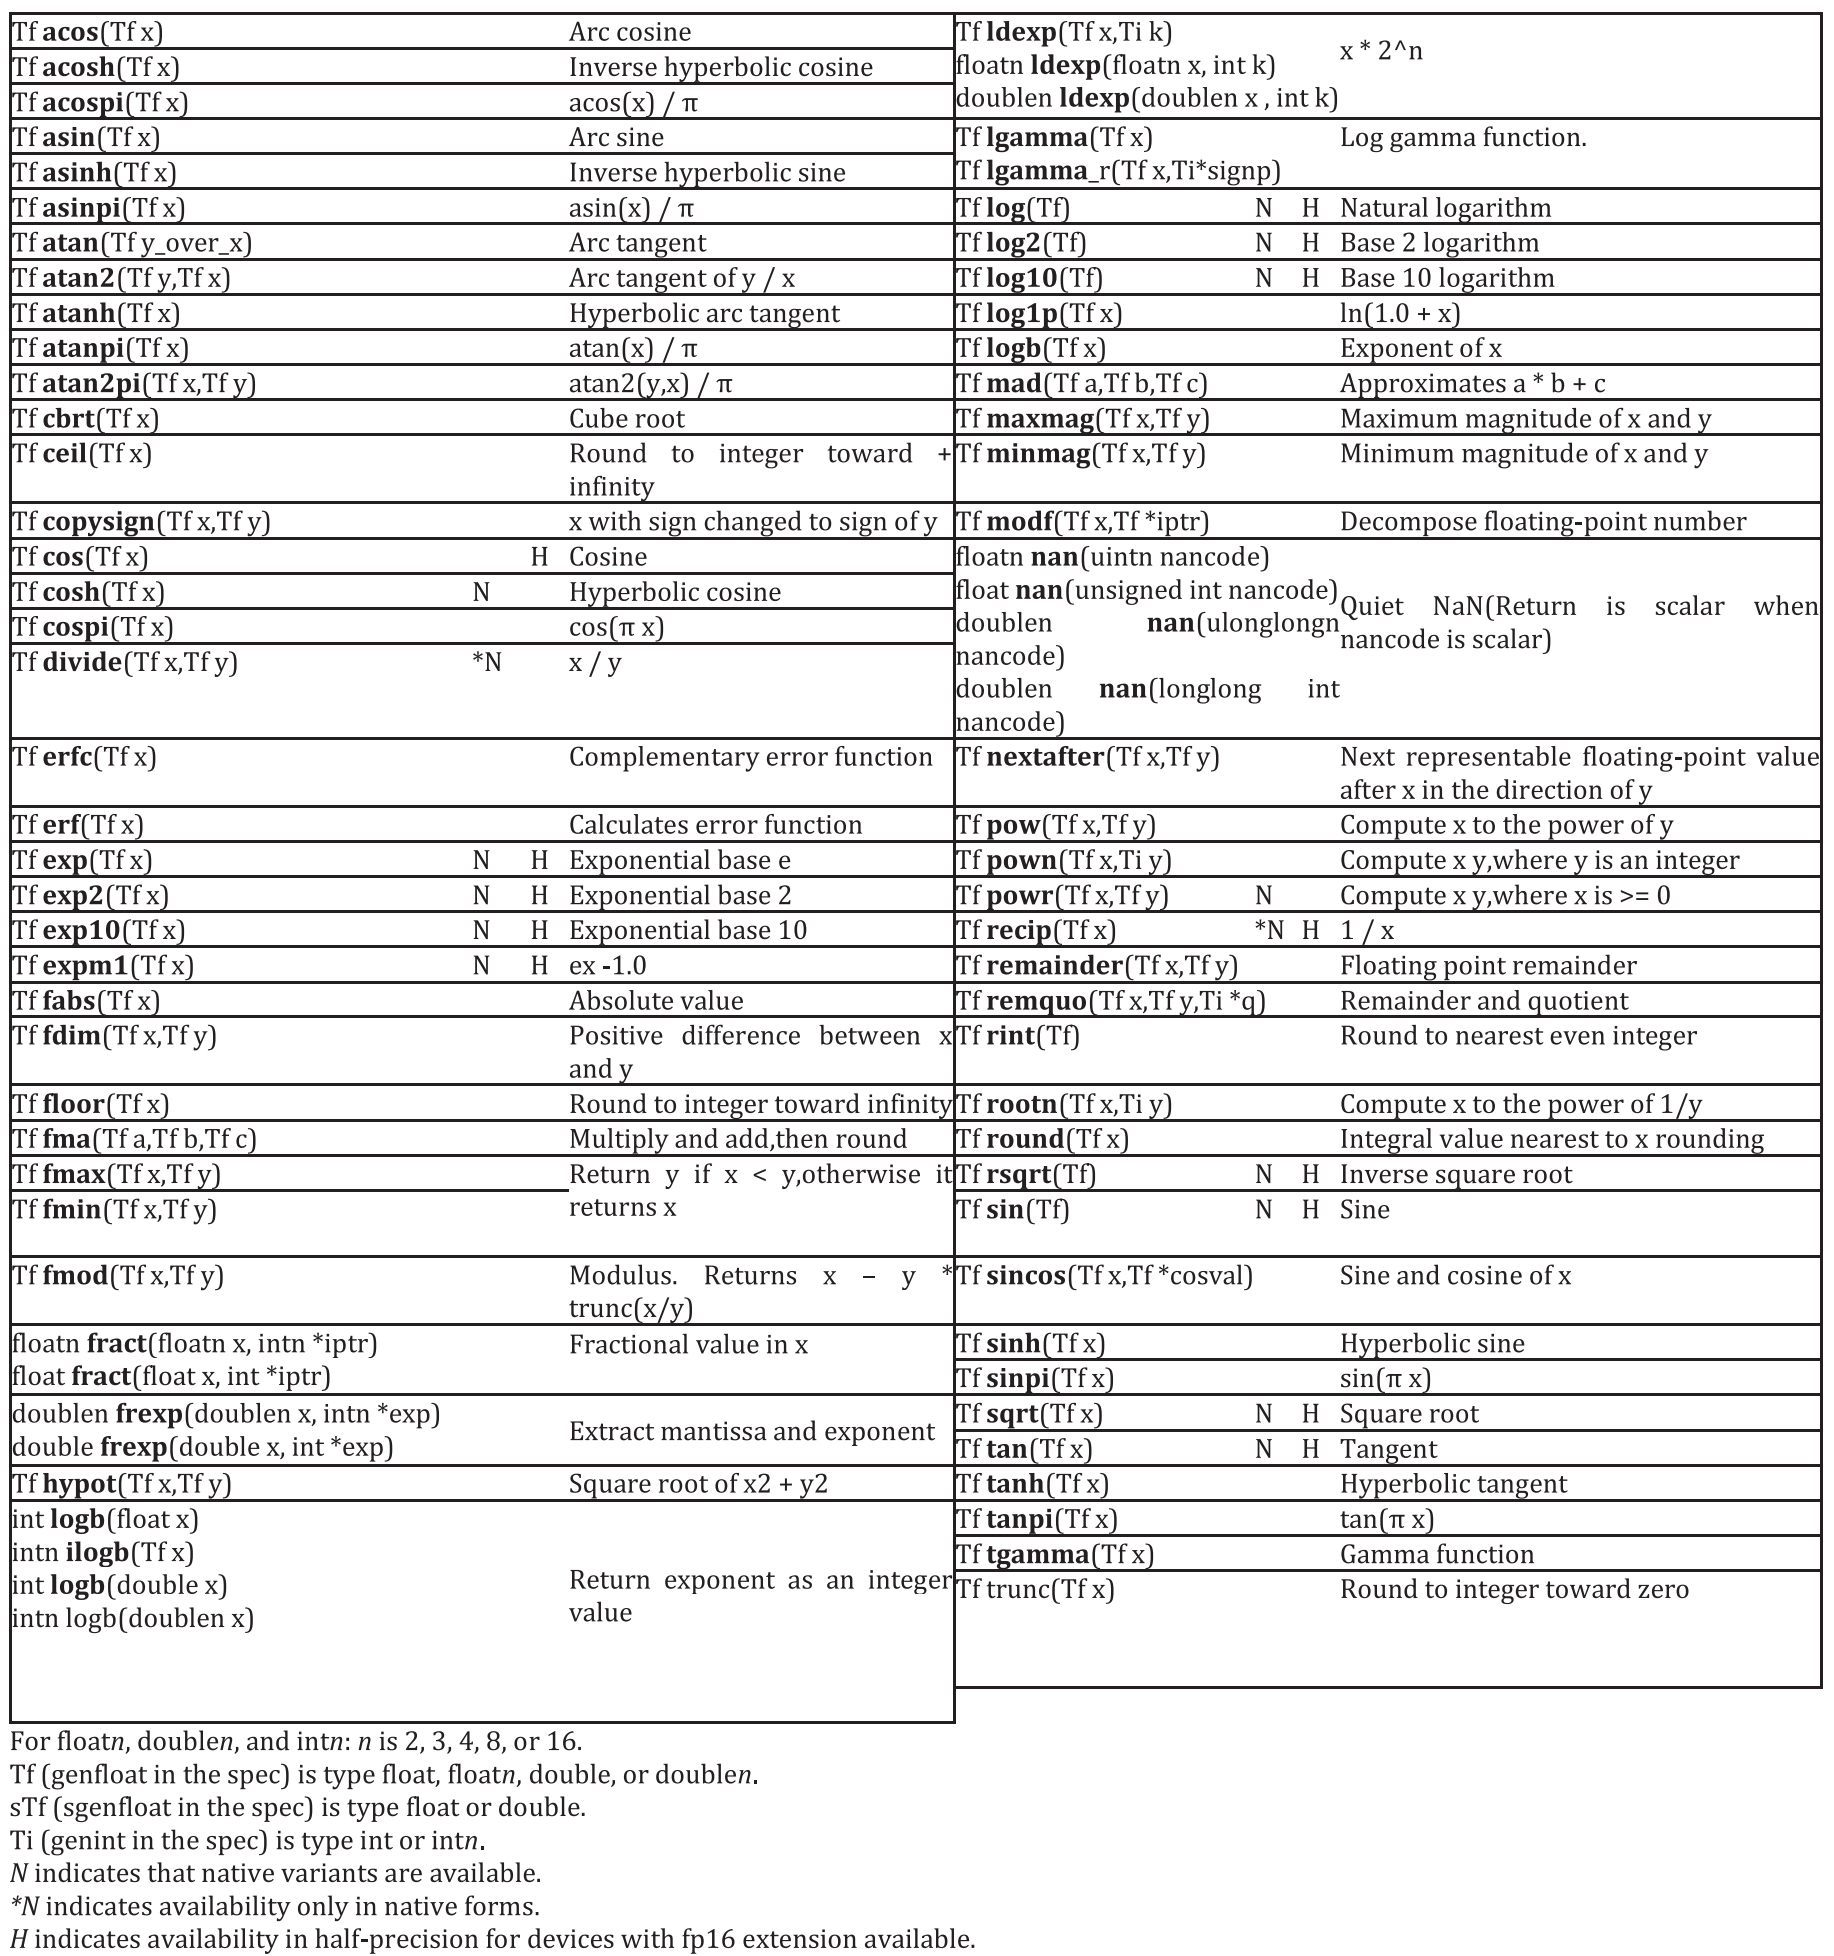
\includegraphics[width=1.0\textwidth]{content/chapter-18/images/2}
\end{center}

\hspace*{\fill} \par %插入空行
Figure 18-3. Built-in integer functions
\begin{center}
	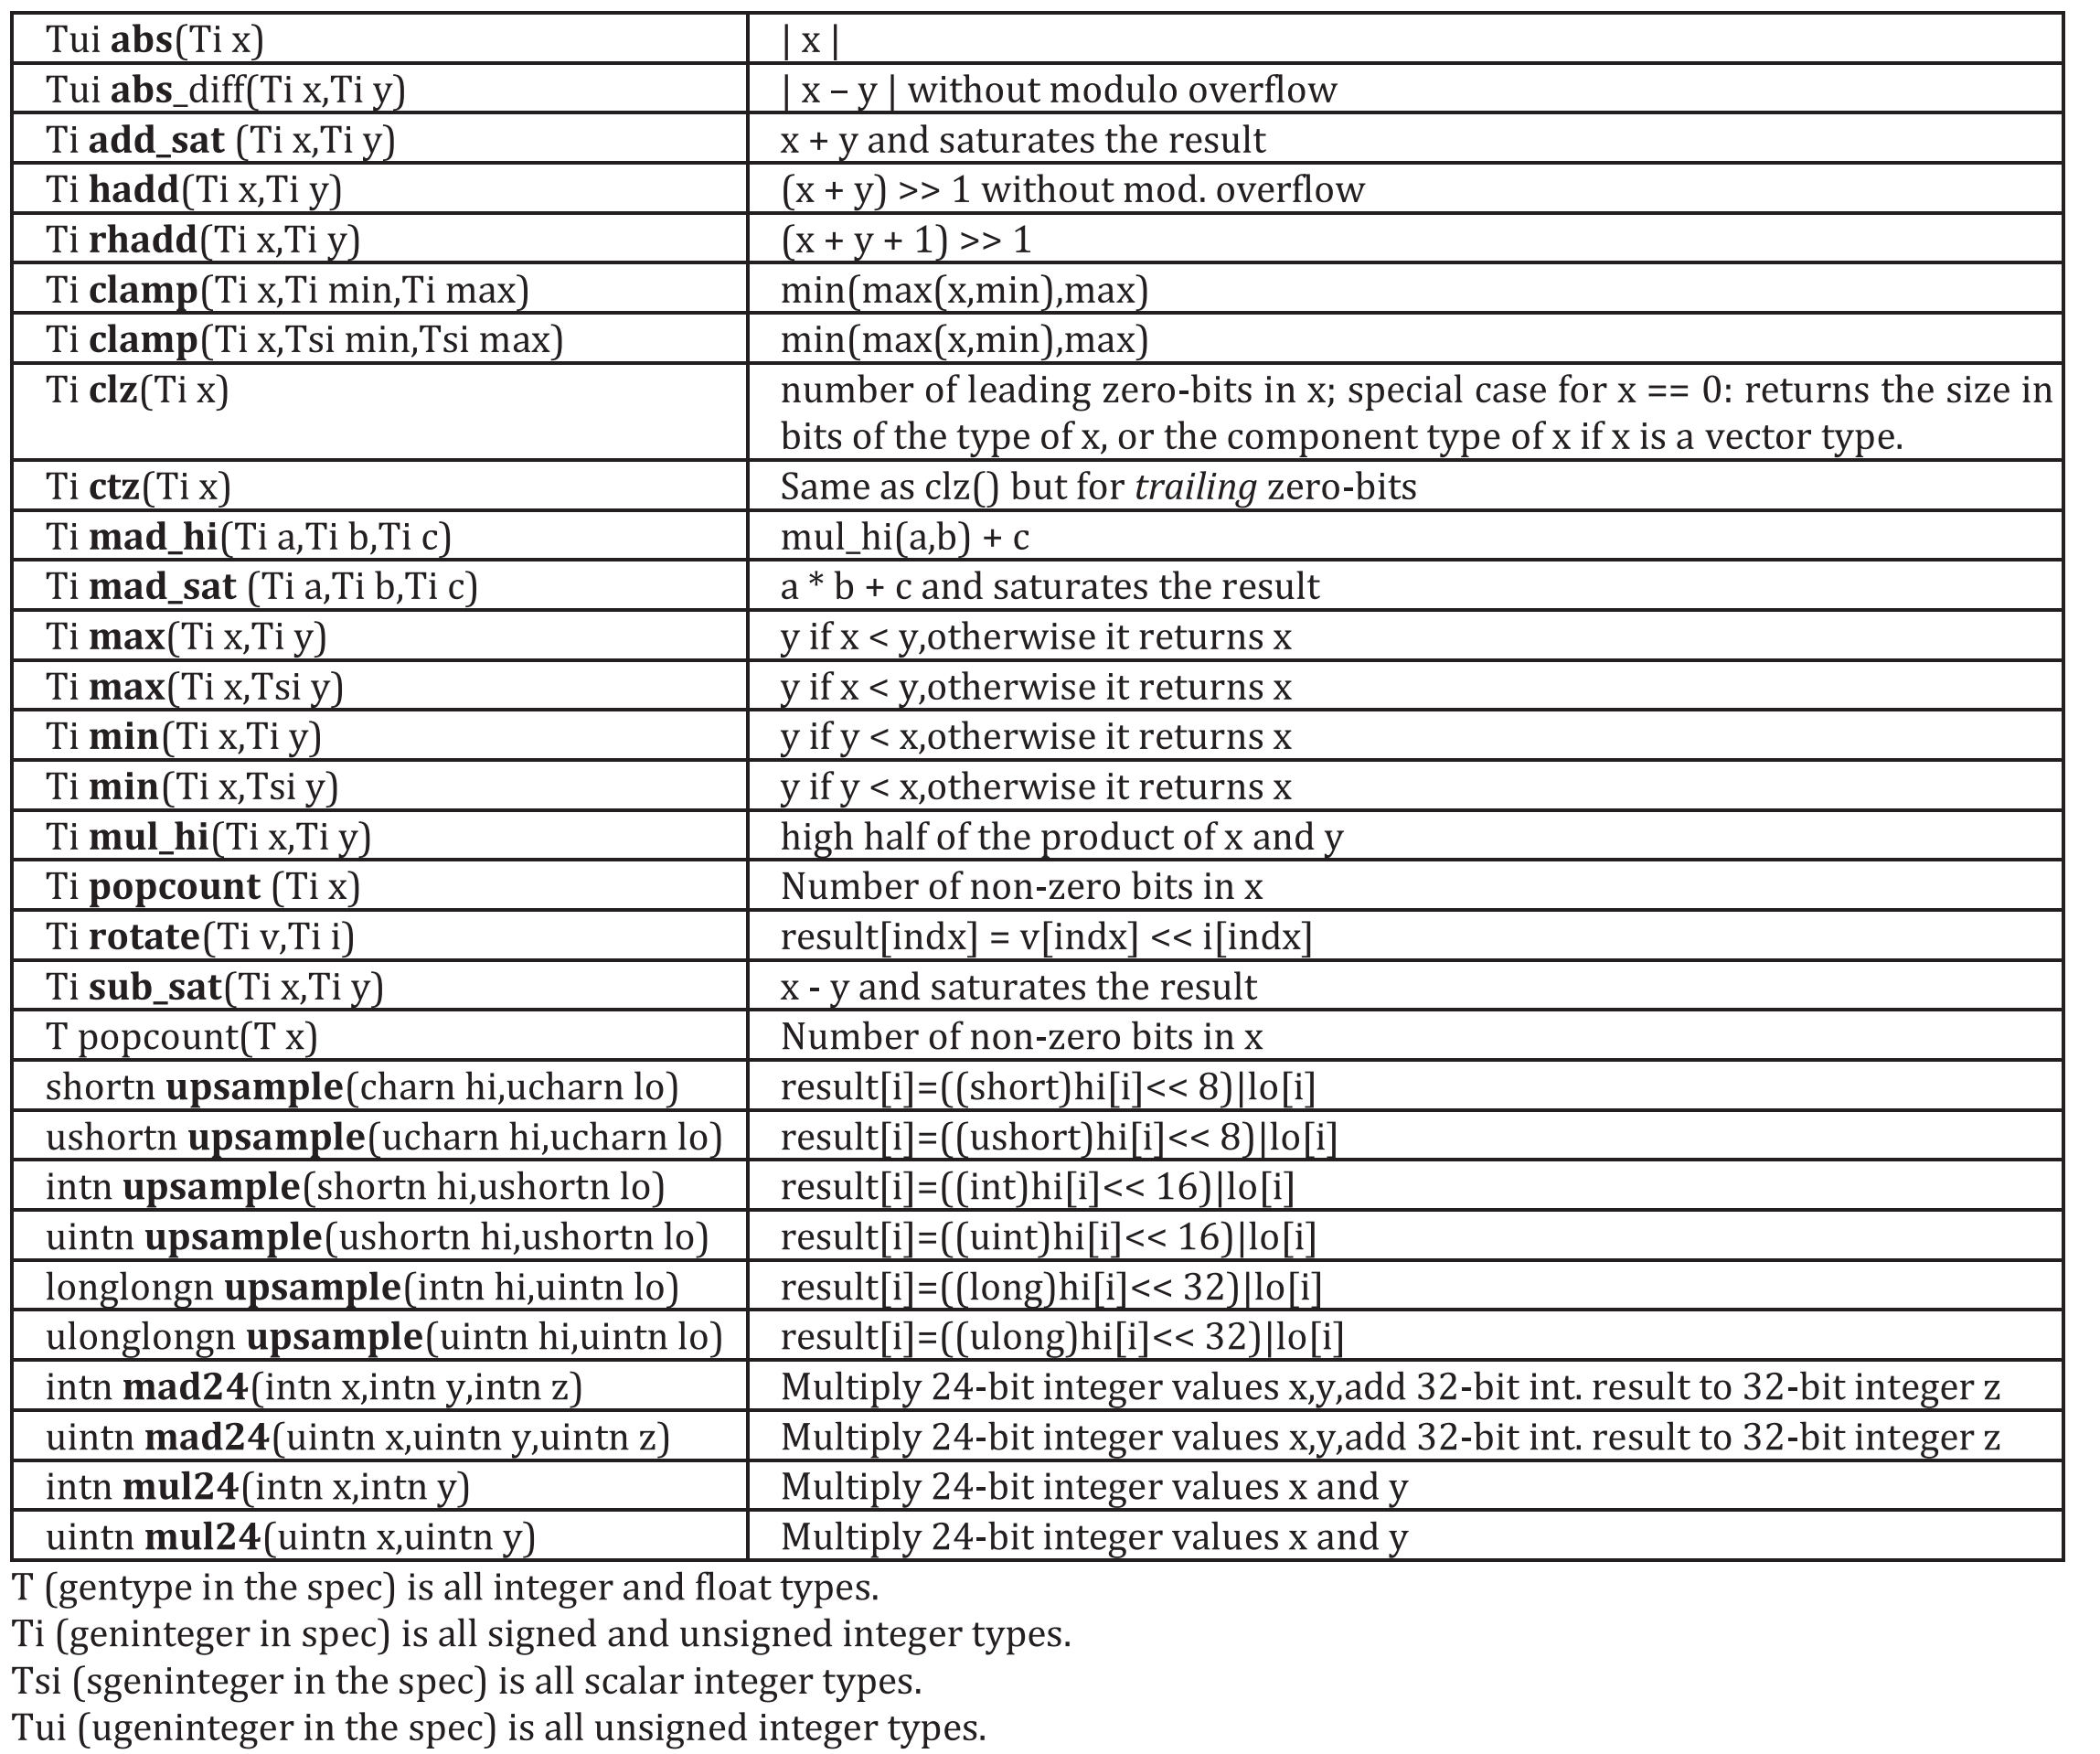
\includegraphics[width=1.0\textwidth]{content/chapter-18/images/3}
\end{center}

\hspace*{\fill} \par %插入空行
Figure 18-4. Built-in common functions
\begin{center}
	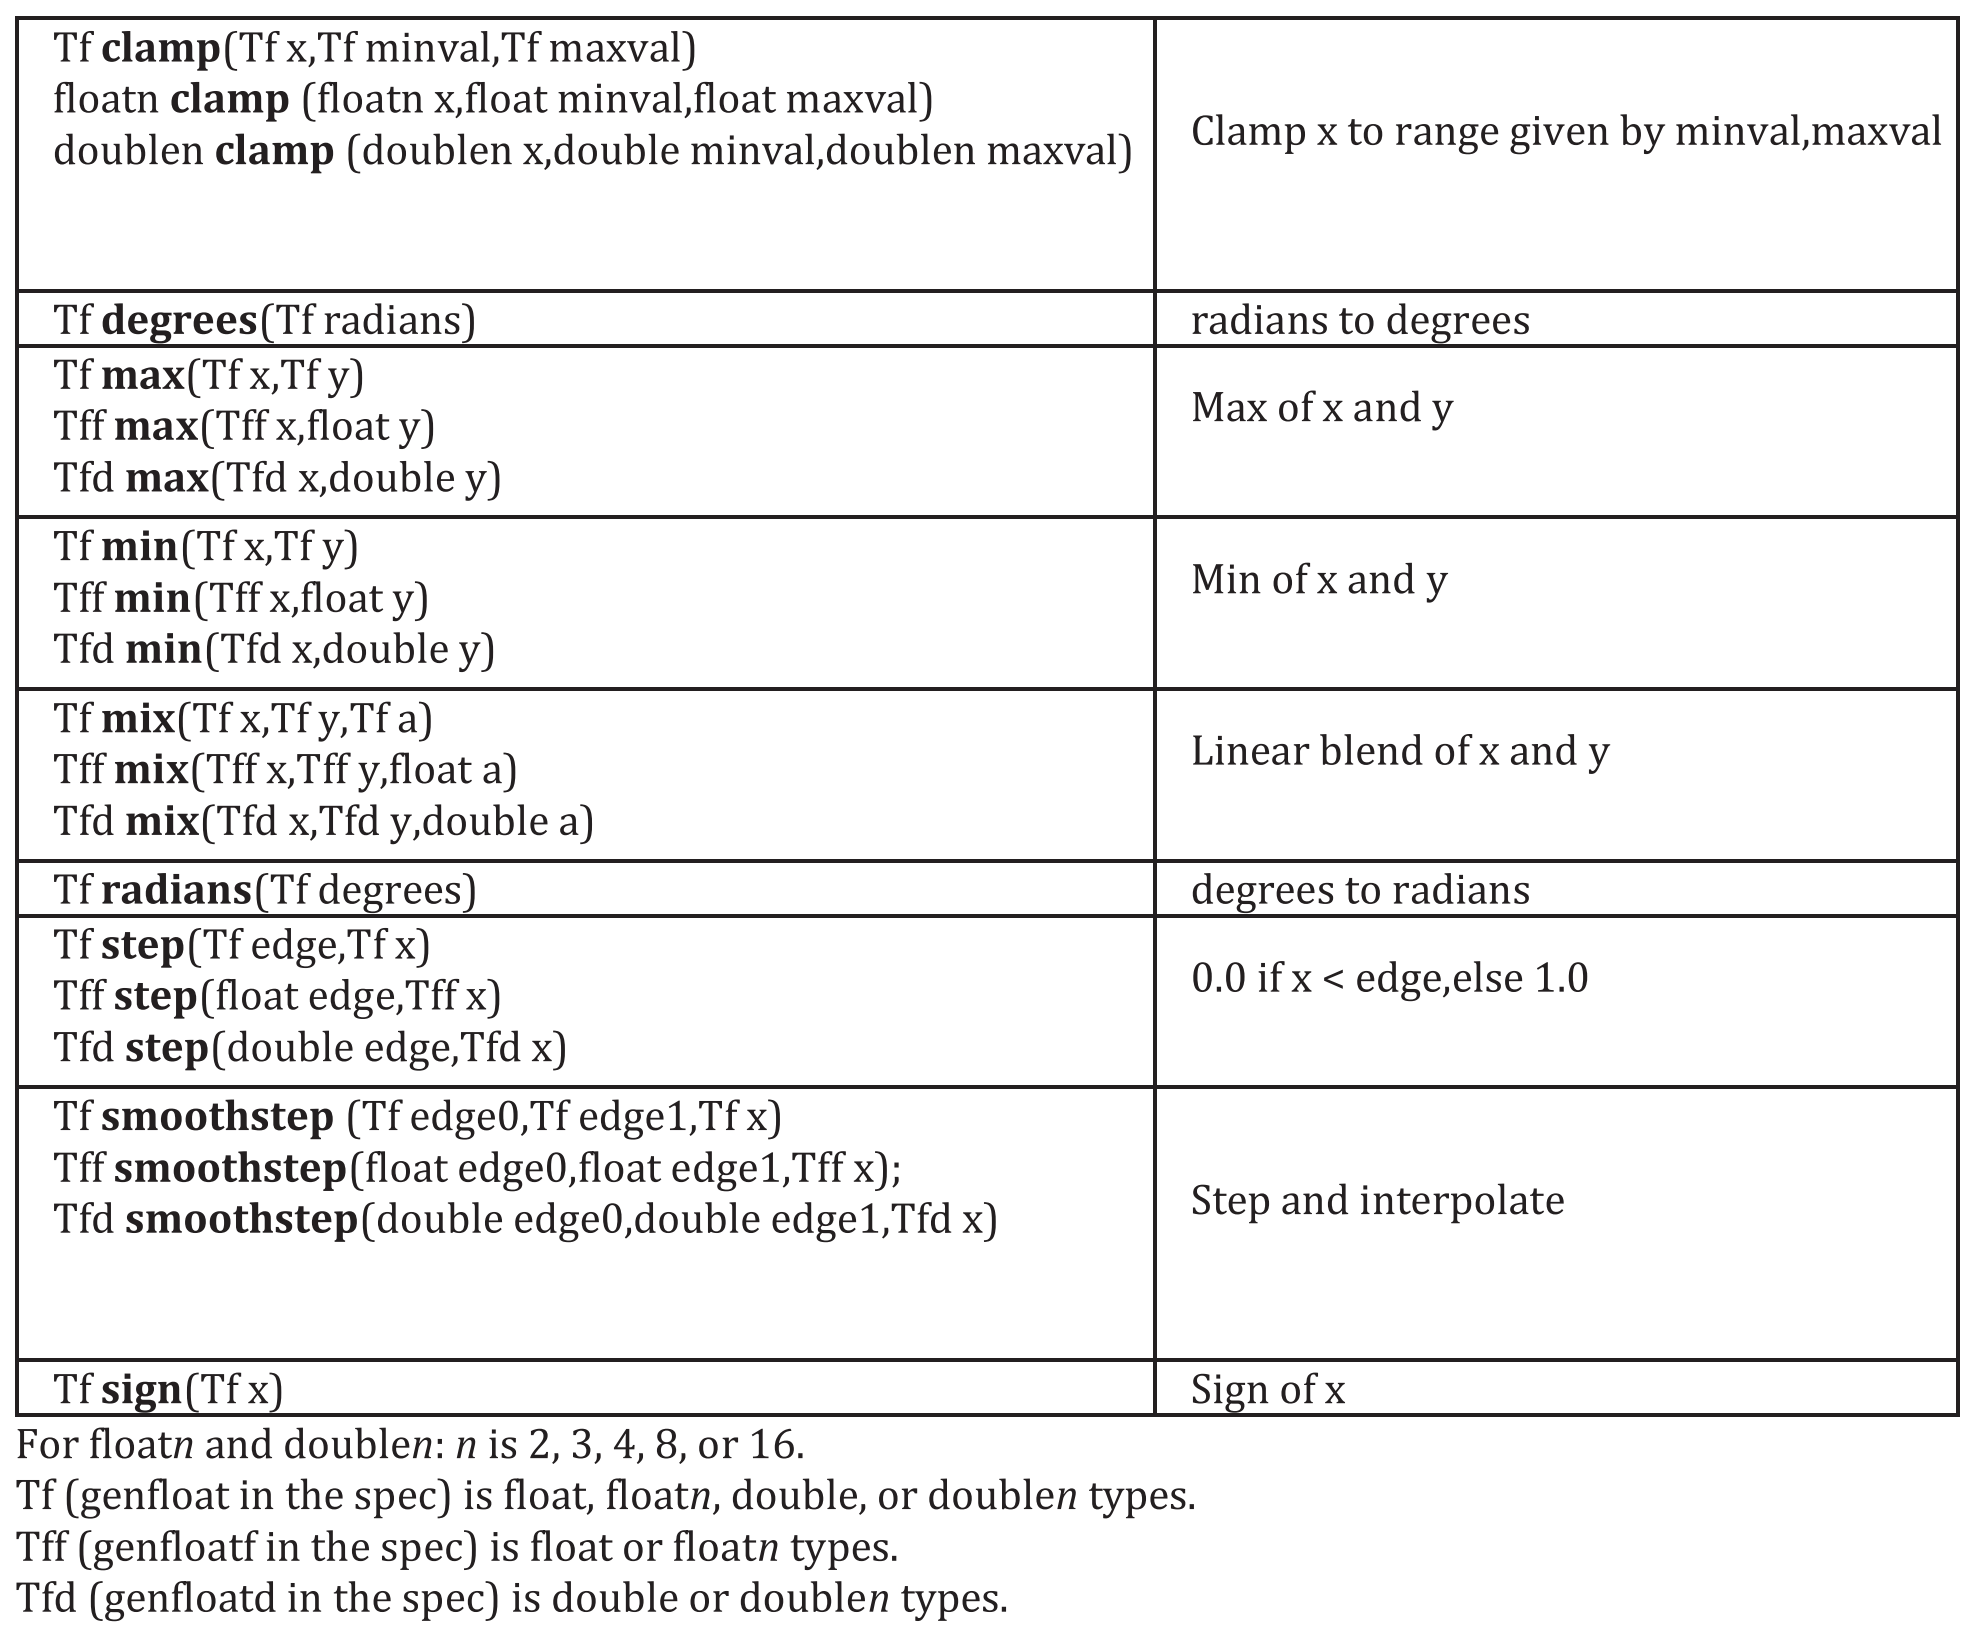
\includegraphics[width=1.0\textwidth]{content/chapter-18/images/4}
\end{center}

\hspace*{\fill} \par %插入空行
Figure 18-5. Built-in geometric functions
\begin{center}
	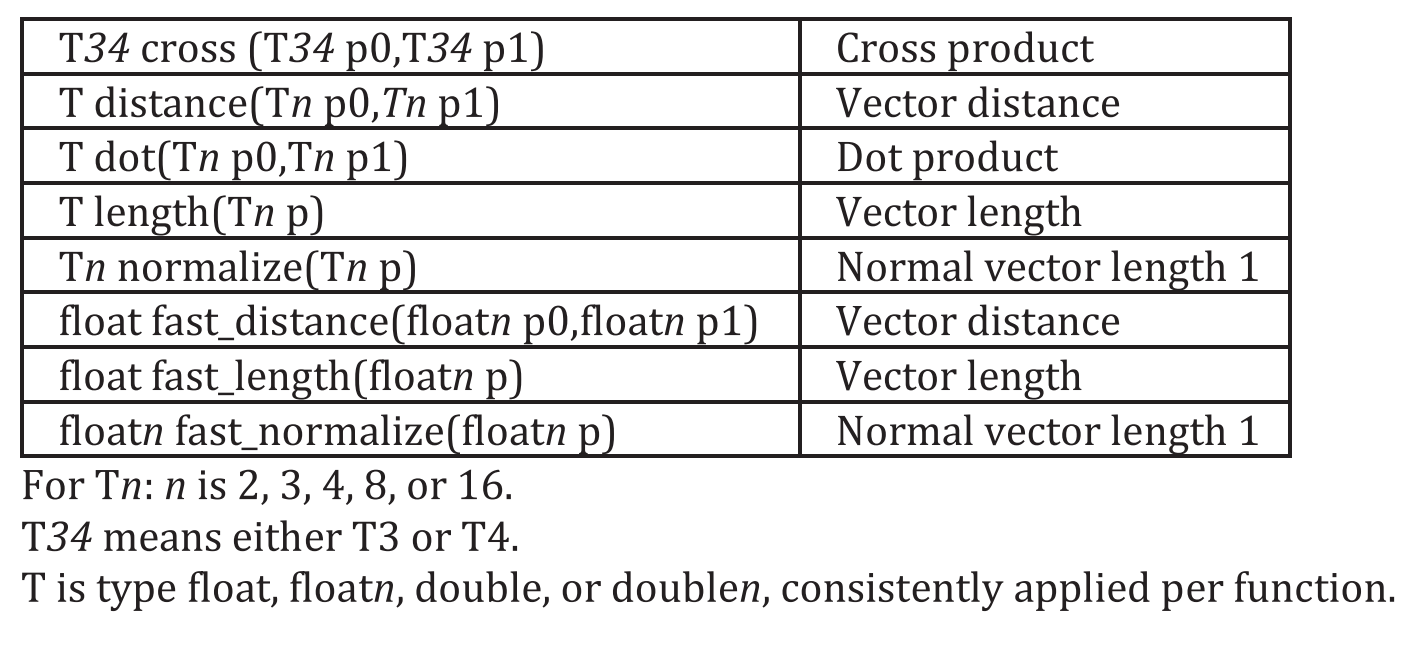
\includegraphics[width=1.0\textwidth]{content/chapter-18/images/5}
\end{center}

\hspace*{\fill} \par %插入空行
Figure 18-6. Built-in relational functions
\begin{center}
	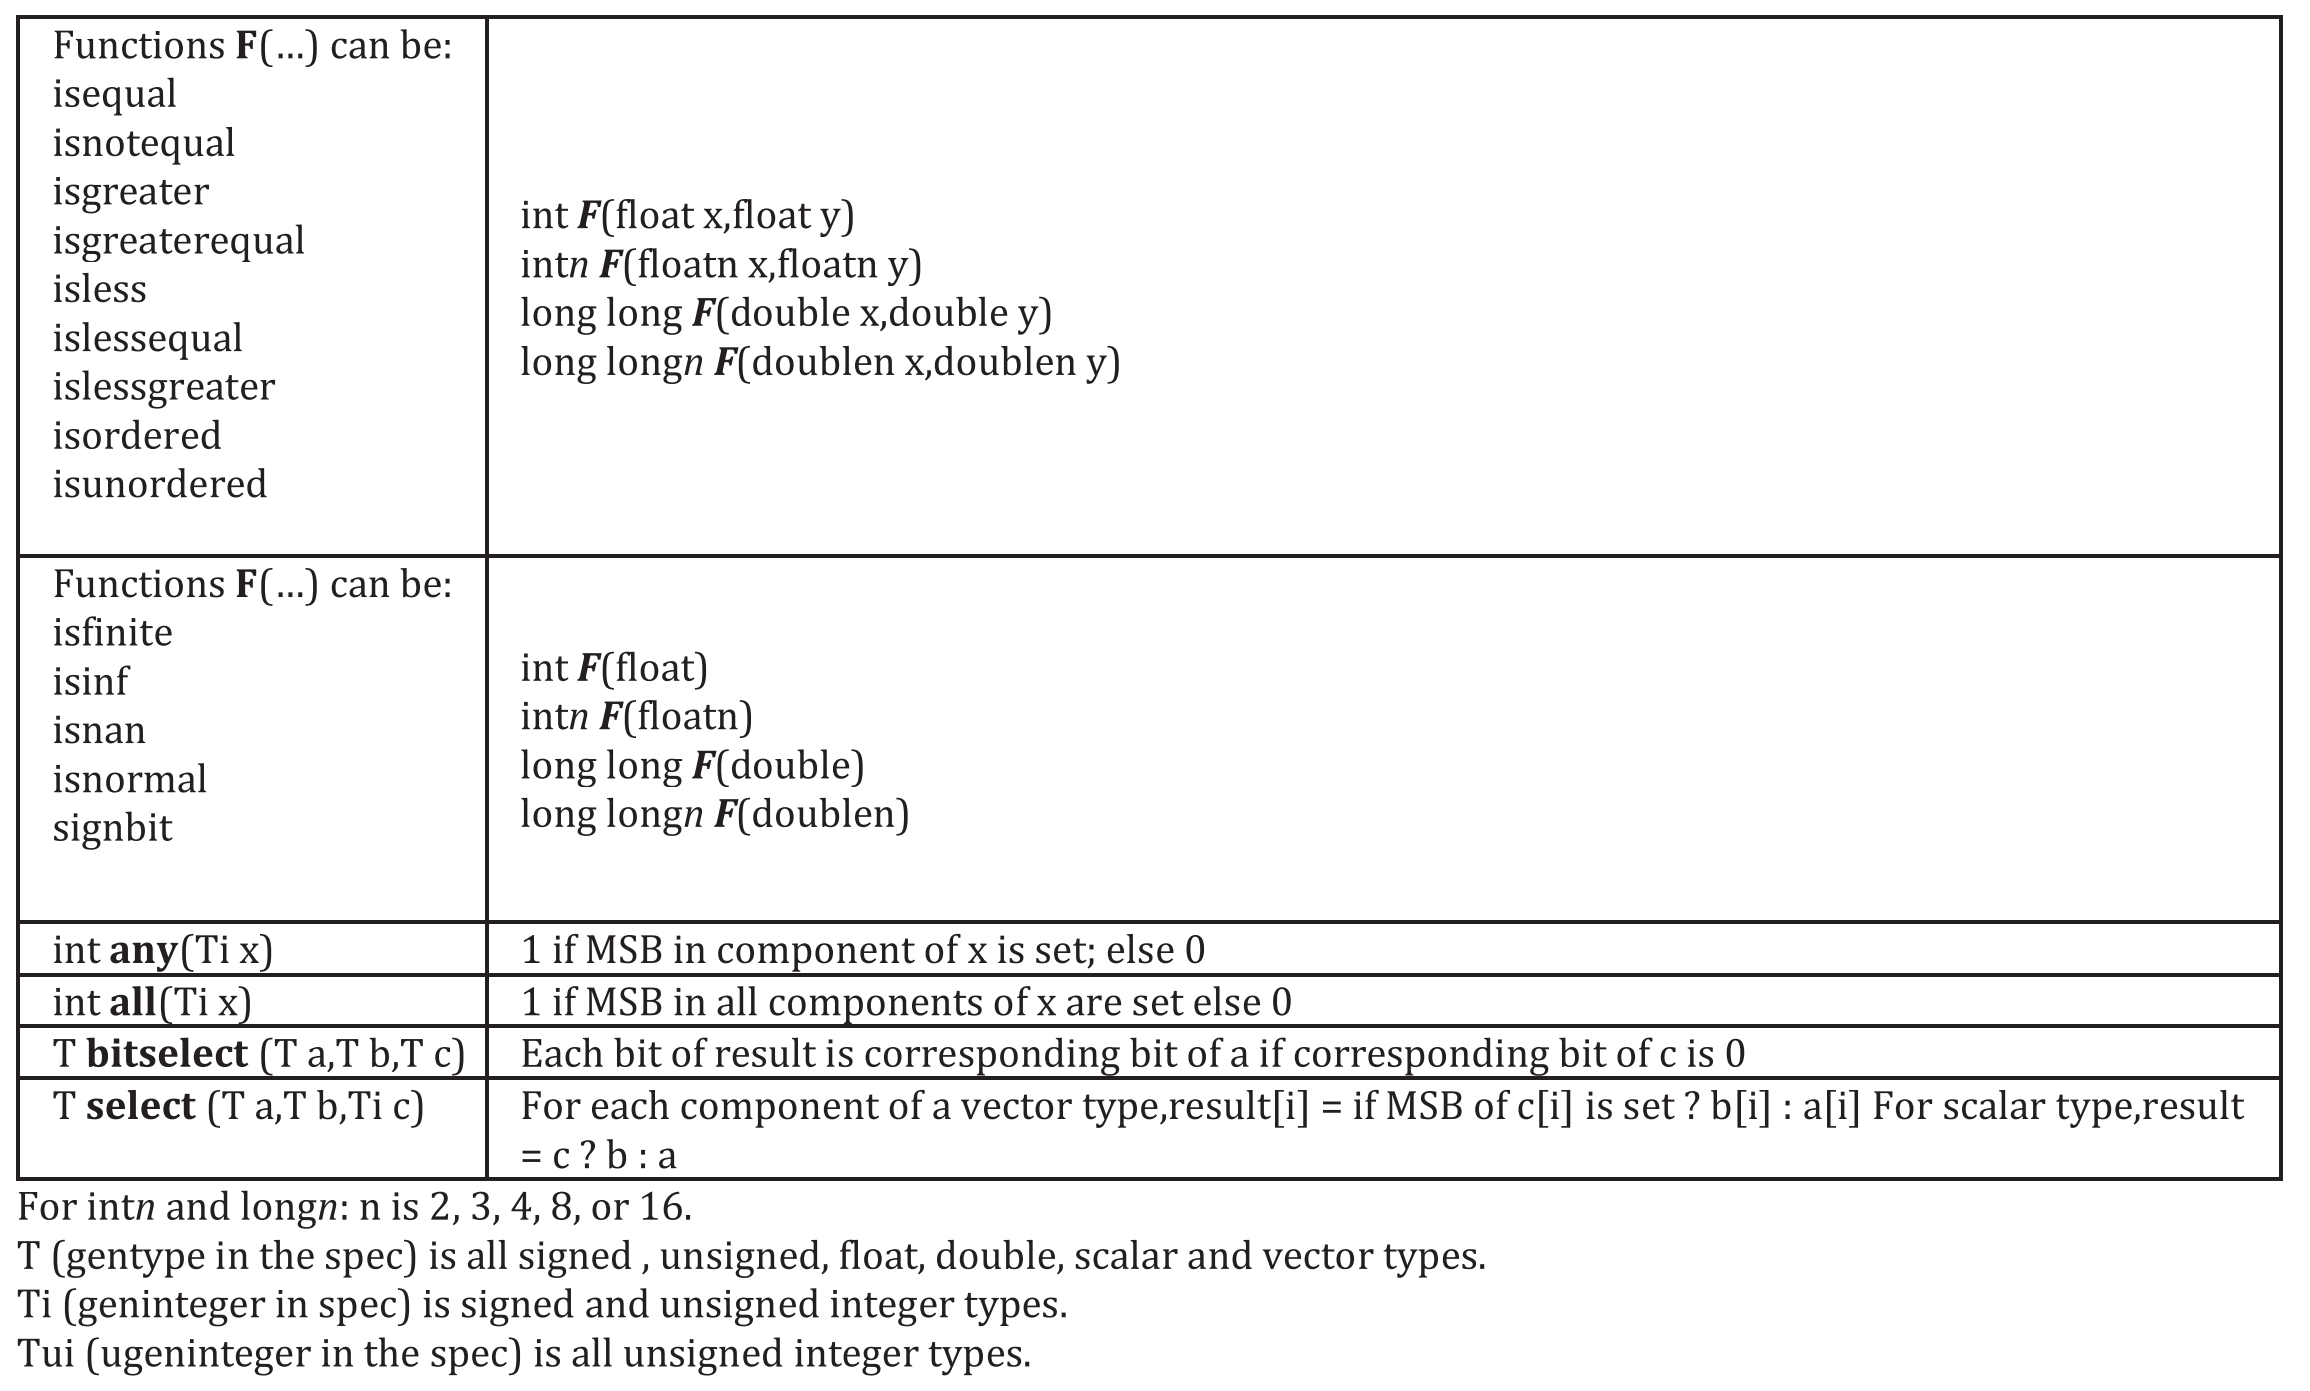
\includegraphics[width=1.0\textwidth]{content/chapter-18/images/6}
\end{center}




























































